\documentclass[a4paper, 12pt, titlepage]{article}

\usepackage[utf8]{inputenc}
\usepackage{geometry}
\usepackage{polski}
\usepackage{graphicx}
\usepackage{float}
\usepackage{etoolbox,refcount}
\usepackage{multicol}
\usepackage{fancyhdr}
\usepackage{listings}
\usepackage{amsmath}
\usepackage{tabularx}
\usepackage{svg}

\pdfsuppresswarningpagegroup=1
\newgeometry{left=2.5cm, right=2.5cm, bottom=2.5cm, top=2.5cm}

\lstset{
    language=Matlab,
    basicstyle=\ttfamily,
    keepspaces=true,
    frame=single,
    tabsize=4,
    showspaces=false,
    showstringspaces=false,
    extendedchars=true,
    inputencoding=utf8,
    literate={ó}{{\'o}}1 {ę}{{\k{e}}}1 {ł}{{\l{}}}1 {ż}{{\.z}}1 {ś}{{\'s}}1 {ć}{{\'c}}1 {ą}{{\k{a}}}1 {ź}{{\'z}}1 {ń}{{\'n}}1
}

\author{Adrian Jałoszewski}
\title{Wstęp do środowiska MATLAB}
\date{9 października 2017}


\begin{document}
    \maketitle
	\section{Cel ćwiczenia}
        Celem ćwiczenia jest zapoznanie się ze środowiskiem MATLAB oraz
        odświeżenie związanej z nim wiedzy.
    \section{Zadanie 1}
        \subsection{Podpunkt a}
\begin{lstlisting}
% Inicjalizacja zmiennych
a = 23;
b = 5;
tmp_max = max(a, b); % Wyznaczenie minimum
tmp_min = min(a, b); % Wyznaczenie maksimum
c = round(tmp_max, tmp_min); % Dzielenie z zaokrągleniem
d = mod(tmp_max, tmp_min); % Reszta z dzielenia
\end{lstlisting}
        \subsection{Podpunkt b}
            Transpozycja wektora wierszowego w celu uzyskania
            kolumnowego:
\begin{lstlisting}
v = [0 5 0 4 0]';
\end{lstlisting}

        \subsection{Podpunkt c}
\begin{lstlisting}
mu = 3; % wartość oczekiwana
sigma = 5; % odchylenie standardowe
R2 = mu + randn(5, 3) * sigma;
\end{lstlisting}

        \subsection{Podpunkt d}
            Konkatenacja wektora z macierzą:
\begin{lstlisting}
v_R2 = [v R2];
\end{lstlisting}

        \subsection{Podpunkt e}
            Wyznaczenie oraz wyrysywanie sinusa:
\begin{lstlisting}
x = 0:pi/10:2*pi;
y = sin(x);
plot(x, y);
\end{lstlisting}
        \begin{figure}[H]
            \centering
            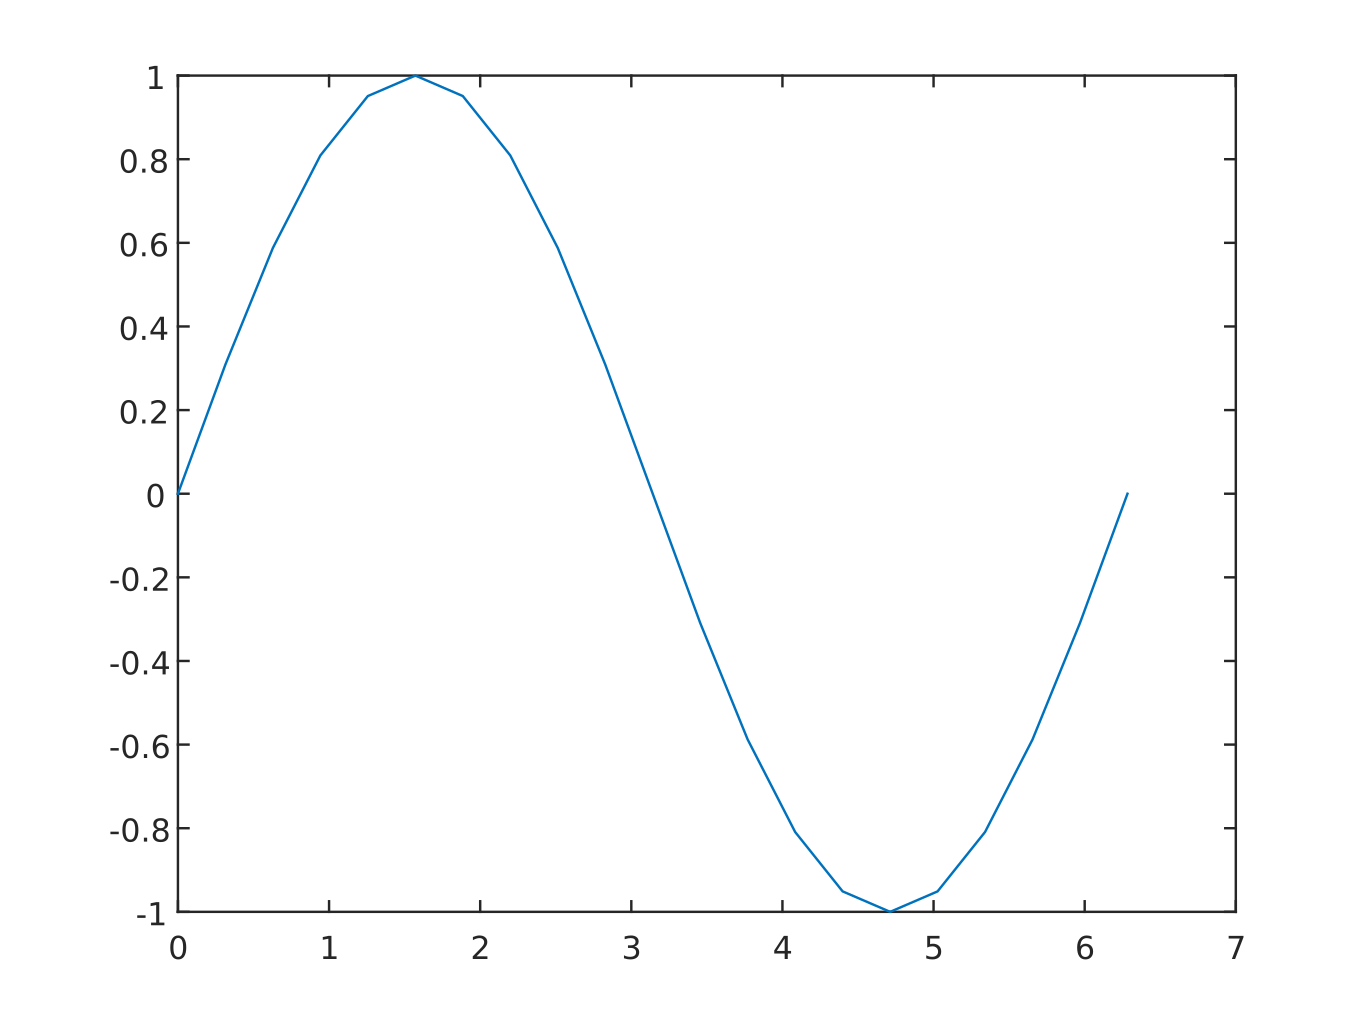
\includegraphics[width=0.8\columnwidth]{sinus.png}
            \caption{Wykres sinusa}
        \end{figure}\noindent

        \subsection{Podpunkt f}
            Wyznaczenie średniej wartości sinusa (bardzo mała, niezerowa)
\begin{lstlisting}
mean(y) % Wynik okazał się być skalarem
\end{lstlisting}
        \subsection{Podpunkt g}
            Zapisanie układu równań w postaci macierzowej:
            $$
                Ax = b
            $$
\begin{lstlisting}
A = [
    1 2 3;
    -1 1 4;
    -1 -2 -3
];

b = [5; 1; -5];

rank_A = rank(A) % macierz źle określona - rząd mniejszy niż 
% x = A \ b

x = pinv(A) * b;
\end{lstlisting}
            Jest zwrócona jedna z możliwych wartości znajdujących się na
            prostej określonej przez układ.
        \subsection{Podpunkt h}
            Wczytanie danych:
\begin{lstlisting}
load('exampledata.mat')
R = RGB(:, :, 1);
G = RGB(:, :, 2);
B = RGB(:, :, 3);
\end{lstlisting}
            Wyświetlenie wczytanych danych z podziałem na poszczególne kolory:
\begin{lstlisting}
subplot(2, 2, 1)
imshow(R);
title('R')

subplot(2, 2, 2)
imshow(G);
title('G')

subplot(2, 2, 3)
imshow(B);
title('B')

subplot(2, 2, 4)
imshow(RGB)
title('RGB')
\end{lstlisting}
        \begin{figure}[H] \centering
            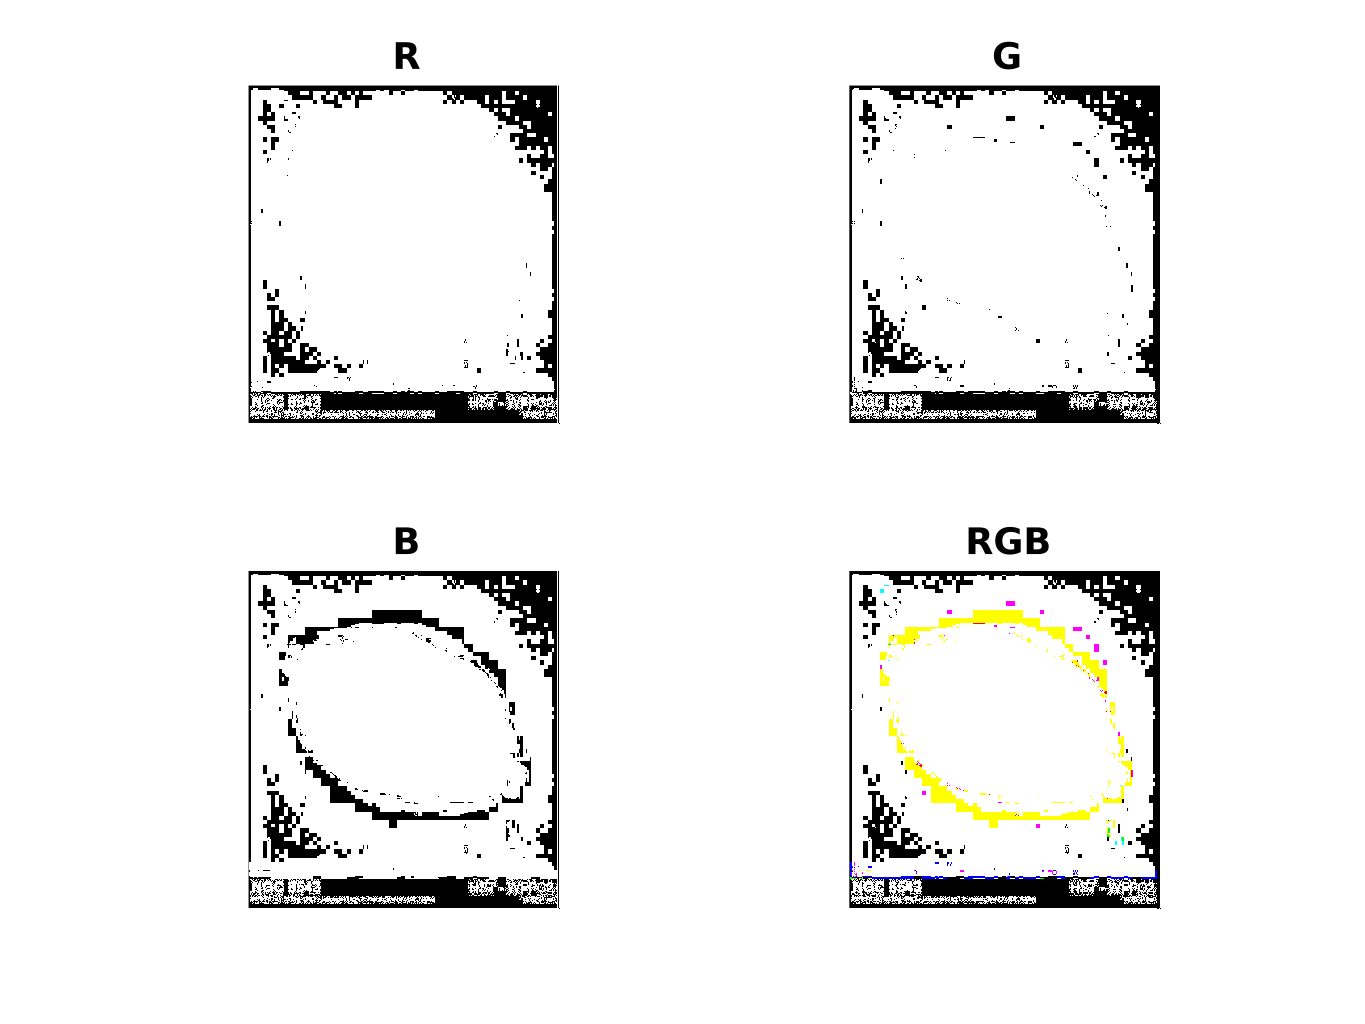
\includegraphics[width=0.8\columnwidth]{RGV.png}
            \caption{Składowe obrazu RGB}
        \end{figure}\noindent
        Zamiana obrazów monochromatycznych kolumnowych na wierszowe i 
        ich konkatenacja w macierz 3xN:
\begin{lstlisting}
R = R(:)';
G = G(:)';
B = B(:)';

ergieb = [R;G;B];
\end{lstlisting}
        Transformacja RGB w YCbCr:
\begin{lstlisting}
b = [
    zeros(1, length(ergieb));
    ones(1, length(ergieb)) * 128;
    ones(1, length(ergieb)) * 128;
];

A = [
    0.299 0.587 0.114;
    -0.169 -0.331 0.5;
    0.5 -0.419 -0.081
];

ycbcr = A * ergieb + b;
\end{lstlisting}
       Zamiana macierzy 3xN na wektory:
\begin{lstlisting}
Y = ycbcr(1, :)';
Cb = ycbcr(2, :)';
Cr = ycbcr(3, :)';
\end{lstlisting}
       Zamiana wektorów na obraz poprzez zmianę ich kształtu:
\begin{lstlisting}
rgb_size = size(RGB);
change_shape = @(y) uint8(reshape(y, rgb_size([1, 2])));

Y = change_shape(Y);
Cb = change_shape(Cb);
Cr = change_shape(Cr);

\end{lstlisting}
       Złożenie obrazu wynikowego ze składowych:
\begin{lstlisting}
YCbCr(:, :, 1) = Y;
YCbCr(:, :, 2) = Cb;
YCbCr(:, :, 3) = Cr;
YCbCr = uint8(YCbCr);
\end{lstlisting}
        Wyświetlenie obrazu YCbCr:
\begin{lstlisting}
figure()
subplot(2, 2, 1)
imshow(Y)
title('Y')

subplot(2, 2, 2)
imshow(Cb)
title('Cb')

subplot(2, 2, 3)
imshow(Cr)
title('Cr')

subplot(2, 2, 4)
imshow(YCbCr)
title('YCbCr')
\end{lstlisting}
        \begin{figure}[H] \centering
            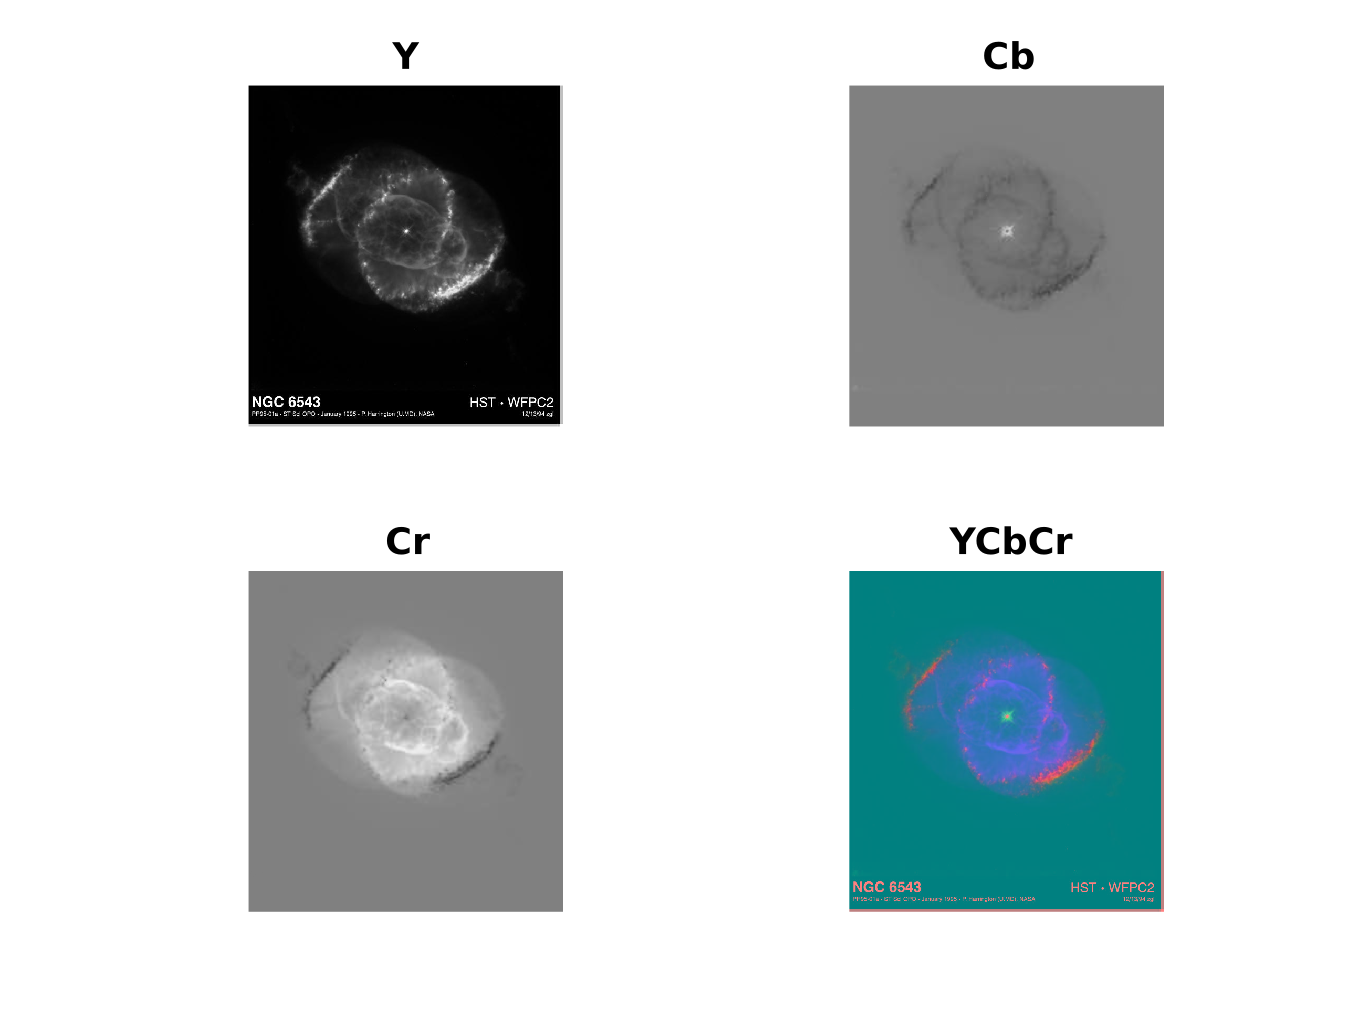
\includegraphics[width=0.8\columnwidth]{YCbCr.png}
            \caption{Składowe obrazu YCbCr}
        \end{figure}\noindent
        \subsection{Podpunkt i}
\begin{lstlisting}
a = pi;
b = ones(1, 1, 'uint8');
c = double(a + b);
\end{lstlisting}
        \subsection{Podpunkt j}
\begin{lstlisting}
abcdefg = 'abcdefg';
% losowe 10 indeksów w zakresie rozmiarów tablicy
rand_int = randi([1, 7], [10, 1]); 
random_characters = abcdefg(rand_int)'
\end{lstlisting}
    
    \section{Zadanie 2}
        \subsection{Podpunkt a}
            Automatycznie wygenerowany kod wczytujący dane z pliku 
            .csv:
\begin{lstlisting}
filename = 'daneP.csv';
delimiter = ',';
startRow = 4;
formatSpec = '%f%f%f%[^\n\r]';
fileID = fopen(filename,'r');
dataArray = textscan(fileID, formatSpec, 'Delimiter', ...
    delimiter, 'HeaderLines' ,startRow-1, 'ReturnOnError', ...
    false, 'EndOfLine', '\r\n');
fclose(fileID);
R1 = dataArray{:, 1};
G1 = dataArray{:, 2};
B1 = dataArray{:, 3};
clearvars filename delimiter startRow formatSpec fileID ...
    dataArray ans;
\end{lstlisting}
    Poszczególne próbki w zależności od numeru porządkowego:
\begin{lstlisting}
subplot(1, 3, 1)
plot(R1)
title('R1')
axis([1, length(R1), -Inf, Inf])

subplot(1, 3, 2)
plot(G1)
title('G1')
axis([1, length(G1), -Inf, Inf])

subplot(1, 3, 3)
plot(B1)
title('B1')
axis([1, length(B1), -Inf, Inf])
\end{lstlisting}
            \begin{figure}[H]
                \centering
                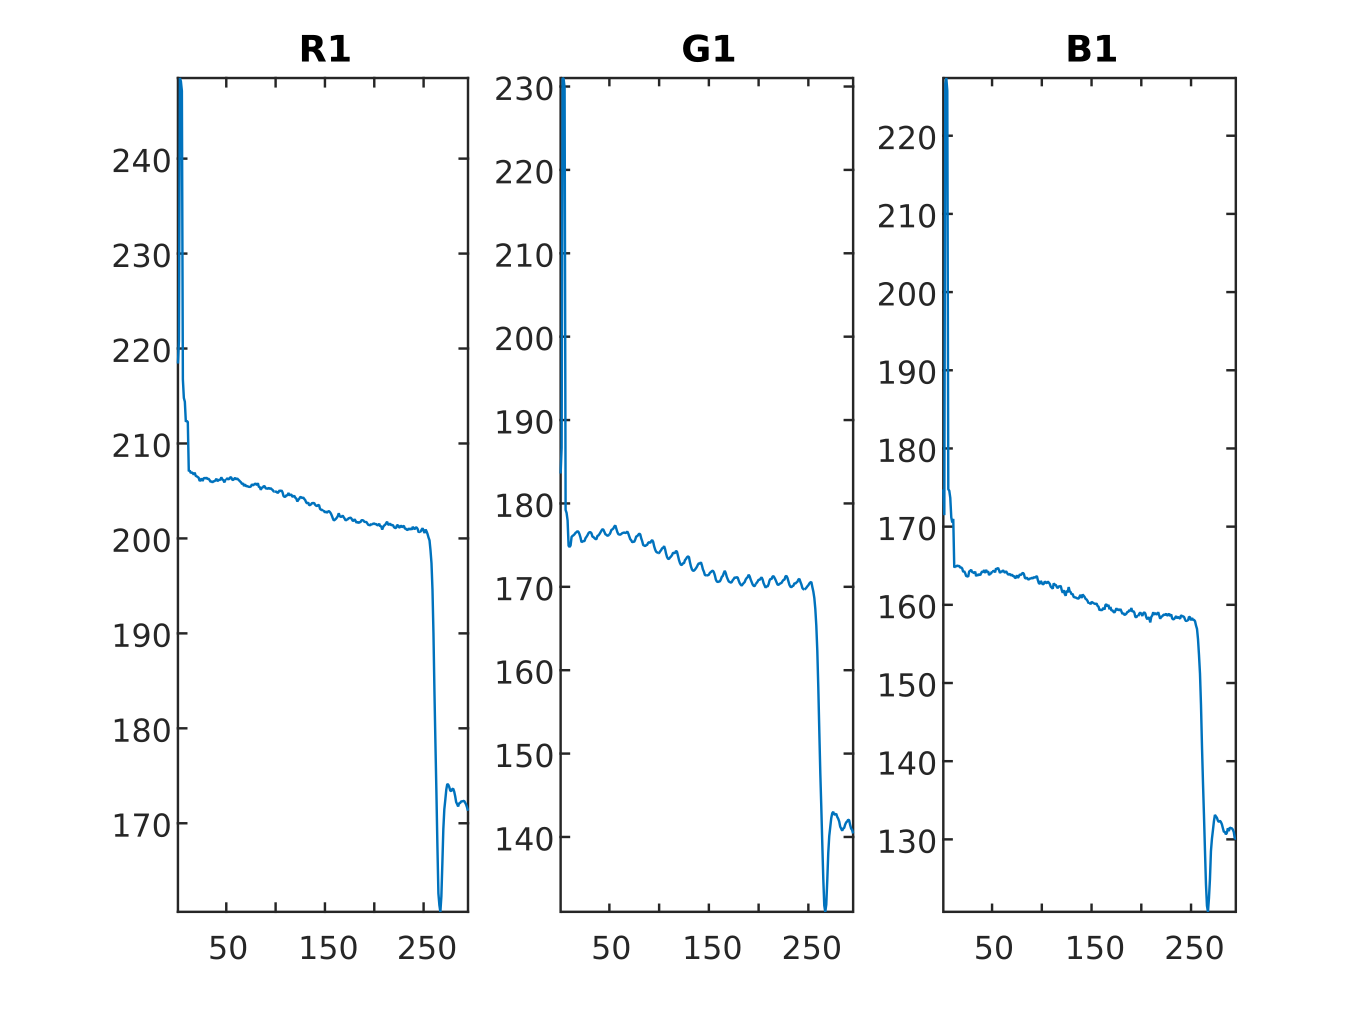
\includegraphics[width=0.8\columnwidth]{read.png}
                \caption{Składowe RGB}
            \end{figure}\noindent
        \subsection{Podpunkt b}
            Przy pomocy narzędzia do pobierania danych graficznie
            znalazłem fragment cykliczny:
\begin{lstlisting}
figure()
periodic_data_R = R1(10:250);
periodic_data_G = G1(10:250);
periodic_data_B = B1(10:250);

subplot(1, 3, 1)
plot(periodic_data_R)
title('R1')
axis([1, length(periodic_data_R), -Inf, Inf])

subplot(1, 3, 2)
plot(periodic_data_G)
title('G1')
axis([1, length(periodic_data_G), -Inf, Inf])

subplot(1, 3, 3)
plot(periodic_data_B)
title('B1')
axis([1, length(periodic_data_B), -Inf, Inf])
\end{lstlisting}
            \begin{figure}[H]
                \centering
                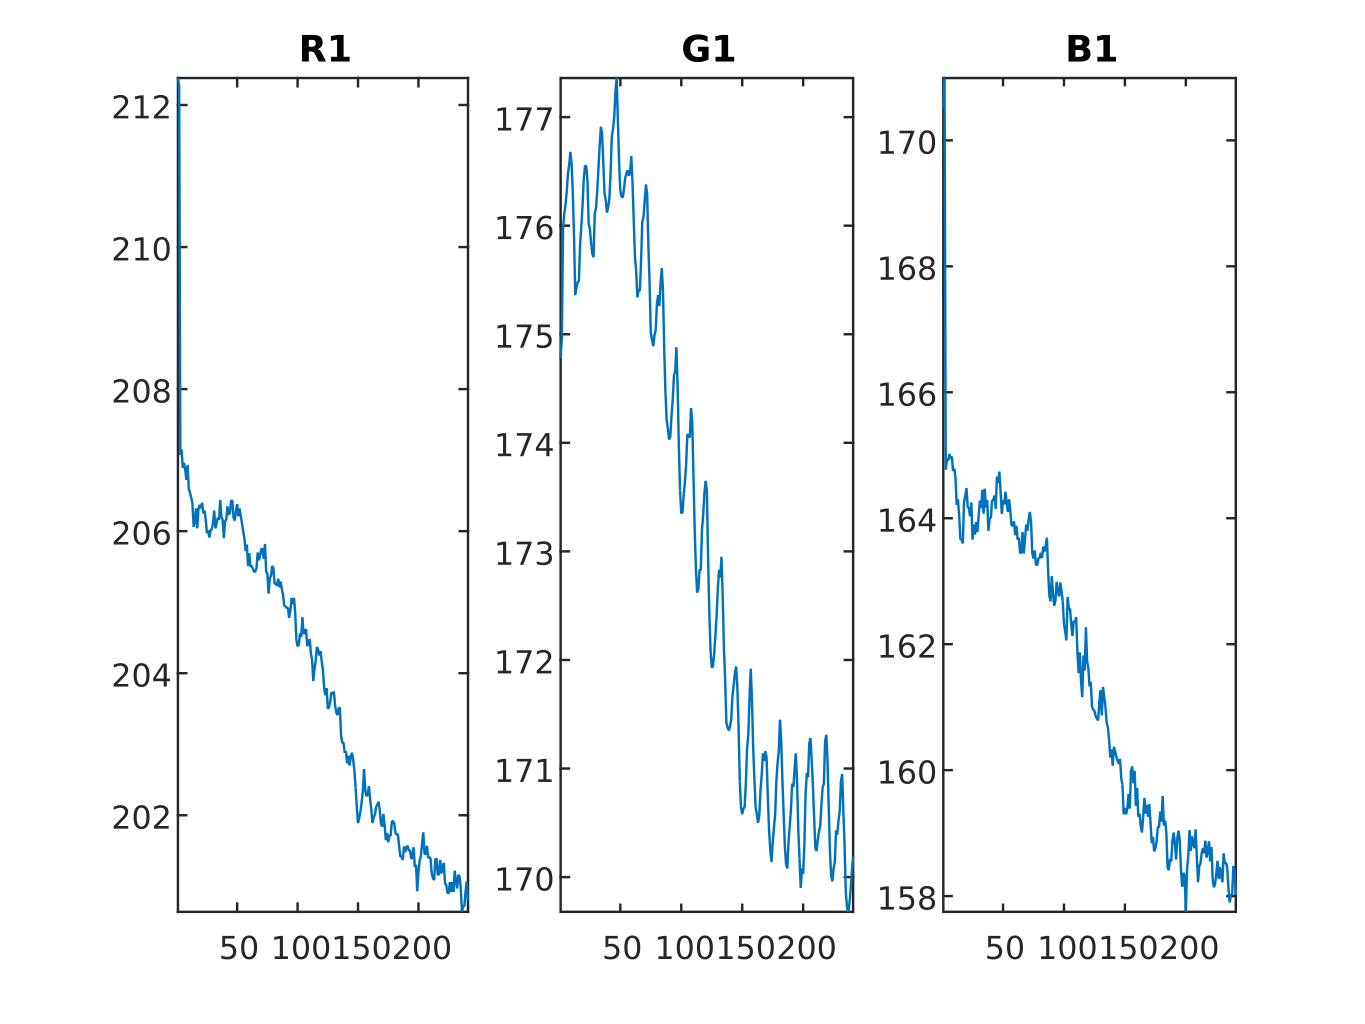
\includegraphics[width=0.8\columnwidth]{periodic.png}
                \caption{Składowe RGB w przedziale okresowości}
            \end{figure}\noindent
            Sygnał okresowy jest najlepiej widoczny w przypadku
            składowej G.
        \subsection{Podpunkt c}
            Dopasowanie trendu na podstawie normy różnicy próbek oraz
            wielomianu aproksymującego.
\begin{lstlisting}
min_delta = 10 ^ 50; % duża liczba
x = 1:length(periodic_data_G);
periodic_data_G = periodic_data_G';

for i = 1:200
    p = polyfit(x, periodic_data_G, i);
    y = polyval(p, x);
    trendles_G = periodic_data_G - y;
    delta = sum((periodic_data_G - y).^2);
    if (delta < min_delta) 
        % jeżeli nowe mnimum - nadpisz minimalne wartości
        min_trendles_G = trendles_G; % składowa G bez trendu
        min_delta = delta; % norma różnicy
        min_poly = y; % wartości wielomianu
        min_degree = i; % rząd wielomianu
    end
end
\end{lstlisting}
            Wyrysowanie próbek pozbawionych trendu oraz wielomianu:
\begin{lstlisting}
figure()
subplot(1, 2, 1)
plot(min_trendles_G)
axis([1, length(min_trendles_G), -Inf, Inf])
title('Funkcja pozbawiona trendu')

subplot(1, 2, 2)
plot(min_poly)
axis([1, length(min_poly), -Inf, Inf])
min_degree % wielomian 32 stopnia
title('Dopasowany wielomian')
\end{lstlisting}
            \begin{figure}[H]
                \centering
                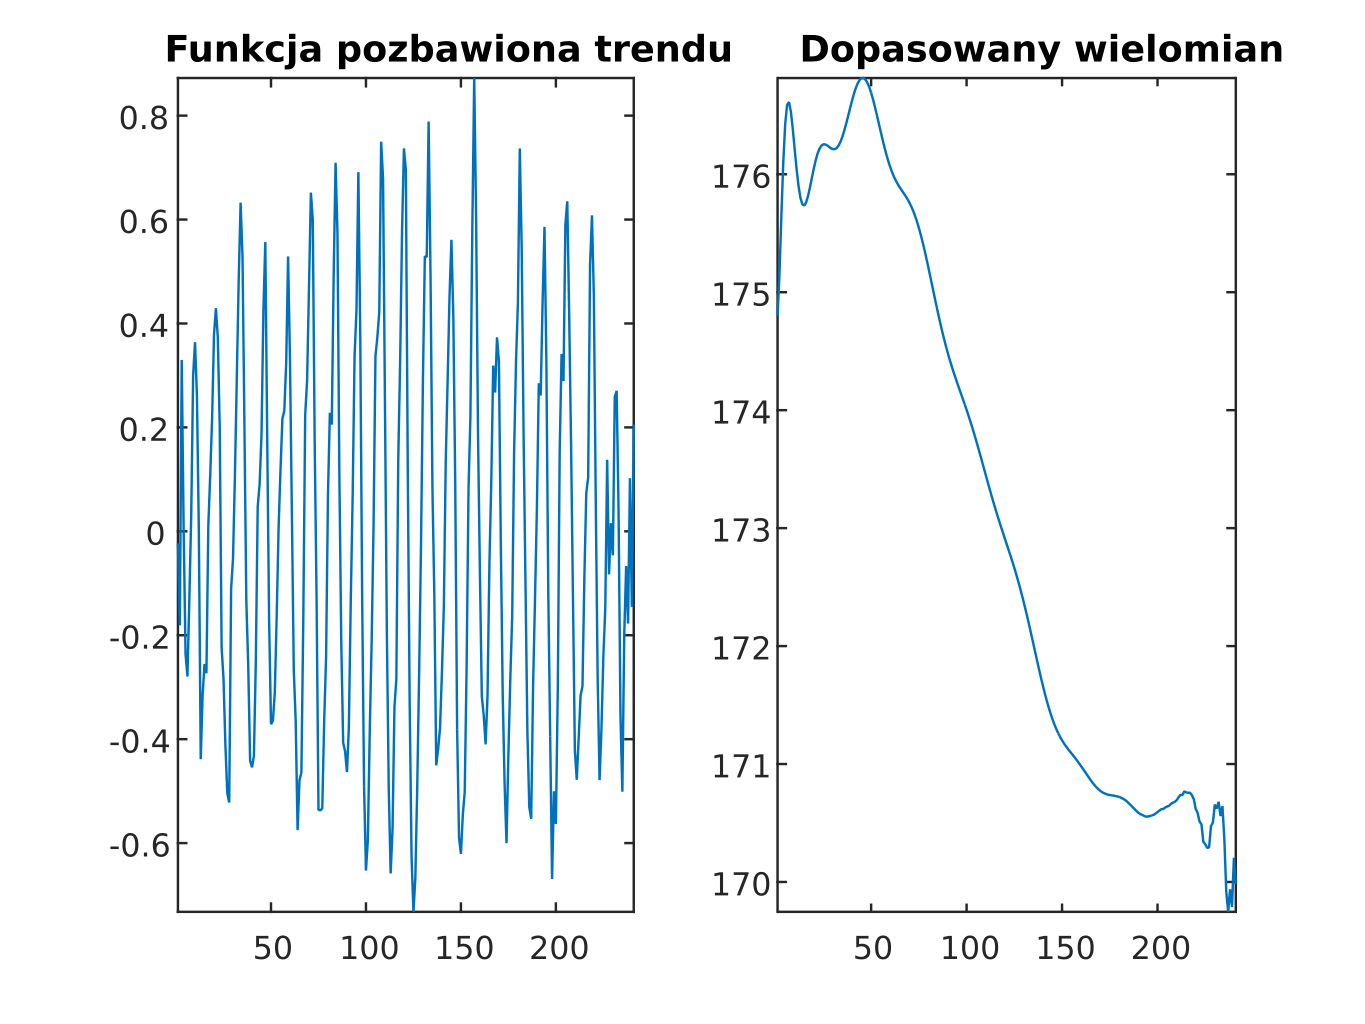
\includegraphics[width=0.8\columnwidth]{polyfit.png}
                \caption{Próbki pozbawione trendu}
            \end{figure}\noindent
        \subsection{Podpunkt d}
            Wyznaczenie transformaty Fouriera:
\begin{lstlisting}
Fs = 60 * 15;                % Sampling frequency                    
T = 1/Fs;                    % Sampling period       
L = length(min_trendles_G);  % Length of signal
t = (0:L-1)*T;               % Time vector

Y = fft(min_trendles_G); % transformata fouriera
P2 = abs(Y/L); % skalowanie oraz moduł z liczb zespolonych
% skalowanie oraz wycięcie częstotliwości ponad połową 
% częstotliwości próbkowania
P1 = P2(1:L/2+1)*2; 
f = Fs * (0:(L/2)) / L; % przeskalowanie częstotliwości
\end{lstlisting}
        Wyrysowanie transformaty Fouriera oraz wyznaczenie maksimum:
\begin{lstlisting}
figure()
plot(f, P1)
axis([0, max(f), 0, max(P1) + 0.1])
title('FFT sygnału')
xlabel('Częstotliwość (Hz)')
ylabel('|Y(f)|')

[x, i] = max(P1) % x = 0.3830
f(i) % 74.69
text(f(i), x, sprintf('\\leftarrow Fc = %d Hz', round(f(i))))
\end{lstlisting}
            \begin{figure}[H]
                \centering
                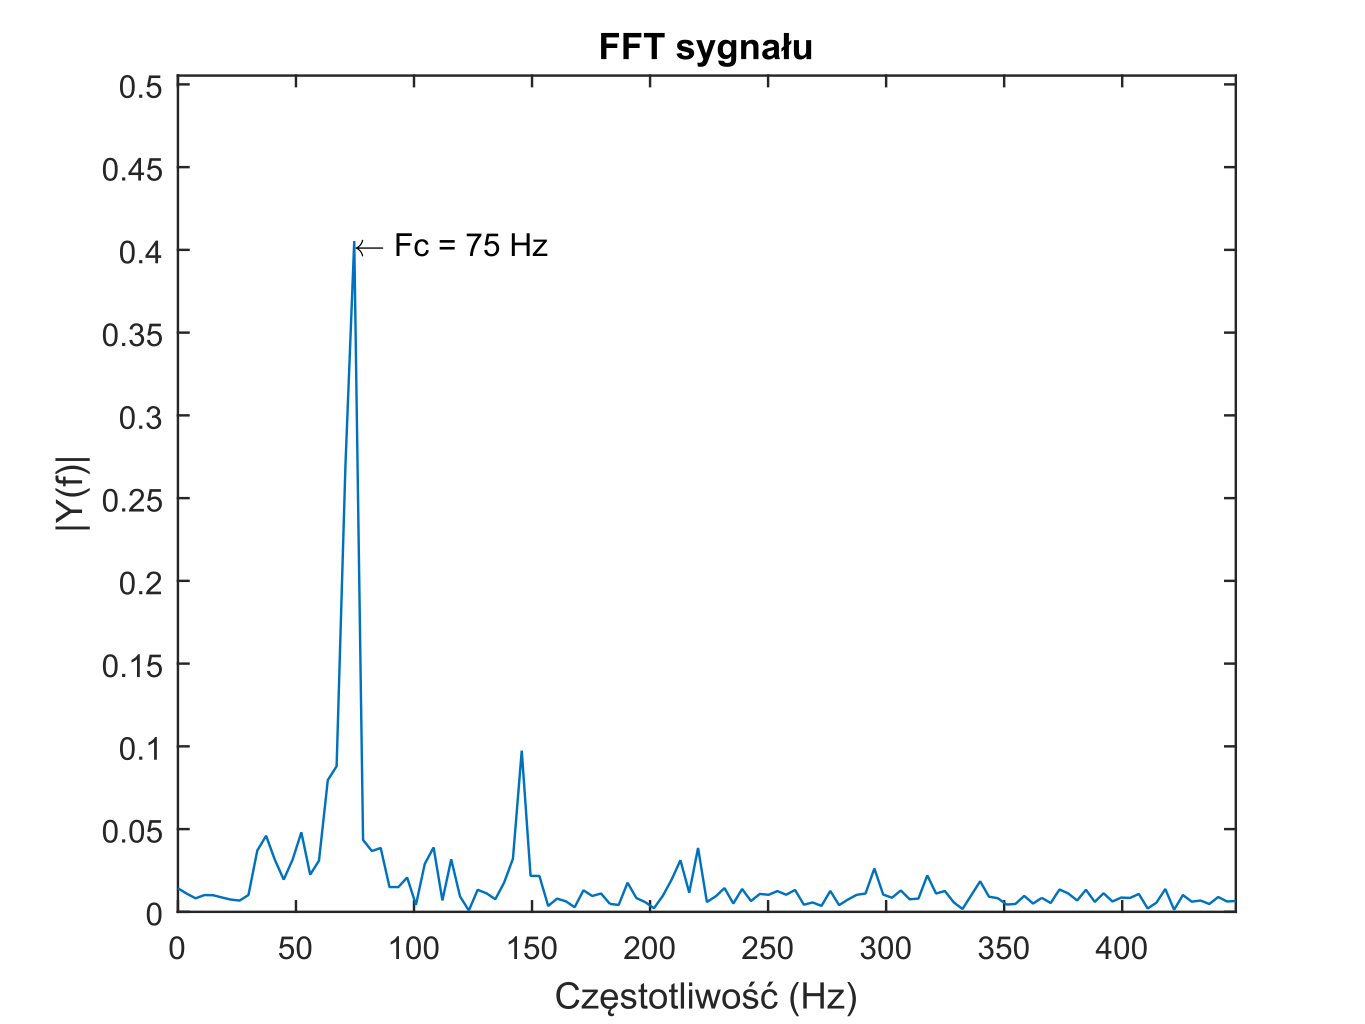
\includegraphics[width=0.8\columnwidth]{FFT.png}
                \caption{Transformata Fouriera dla próbek G1}
            \end{figure}\noindent
    \section{Zadanie 3}
        \subsection{Podpunkt a}
\begin{lstlisting}
% Macierz o rozkładie normalnym i wymiarach 3x3
R = randn(3, 3) 
A = uint32(100) % liczba całkowita 32-bitowa
B = uint32(R * double(A)) % ich mnożenie

a = 1; % 8 bajtów
b = uint32(a); % 4 bajty
whos
\end{lstlisting}

        \subsection{Podpunkt b}
            Stworzenie tablicy dwuwymiarowej stringów (konkatenacja w
            pionie):
\begin{lstlisting}
str1 = 'ćwiczenie 2';
str2 = 'laboratorium 1';
str3 = strvcat(str1, str2)
\end{lstlisting}

        \subsection{Podpunkt c}
            Wyrażenie regularne zaczynające się od ,,b'', kończące na
            ,,d'' i nie posiadające ani ,,u'' ani białych znaków.
\begin{lstlisting}
str1 = ['Krasnoludy przeszły przez rzekę w bród, ' ...
    'nie zamoczywszy swych bród i do tego zmywszy' ...
    ' ze swych nóg brud']
expression = 'b[^u\s]*d'; 
indices = regexp(str1, expression) % 35, 63 
\end{lstlisting}
            Słowa spełniające te wyrażnie regularne znajdują się pod
            indeksami 35 oraz 63.

        \subsection{Podpunkt d}
\begin{lstlisting}
% Utworzenie na podstawie wcześniejszej macierzy R
cell_array = {
    123, 'abcd';
    R, 0.1
}
\end{lstlisting}
                Dodanie 100 do komórki z macierzą R
\begin{lstlisting}
cell_array{2, 1} = cell_array{2, 1} + 100
\end{lstlisting}

        \subsection{Podpunkt e}
\begin{lstlisting}
fn = @(x) x.^2 - 2 * x + 4; % funkcja anonimowa - parabola
integral = quad(fn, -2, 2)  % 21.33 - wartość całki
% wykres funkcji w przedziale [-2, 2]
fplot(fn, [-2, 2])          
\end{lstlisting}
            \begin{figure}[H]
                \centering
                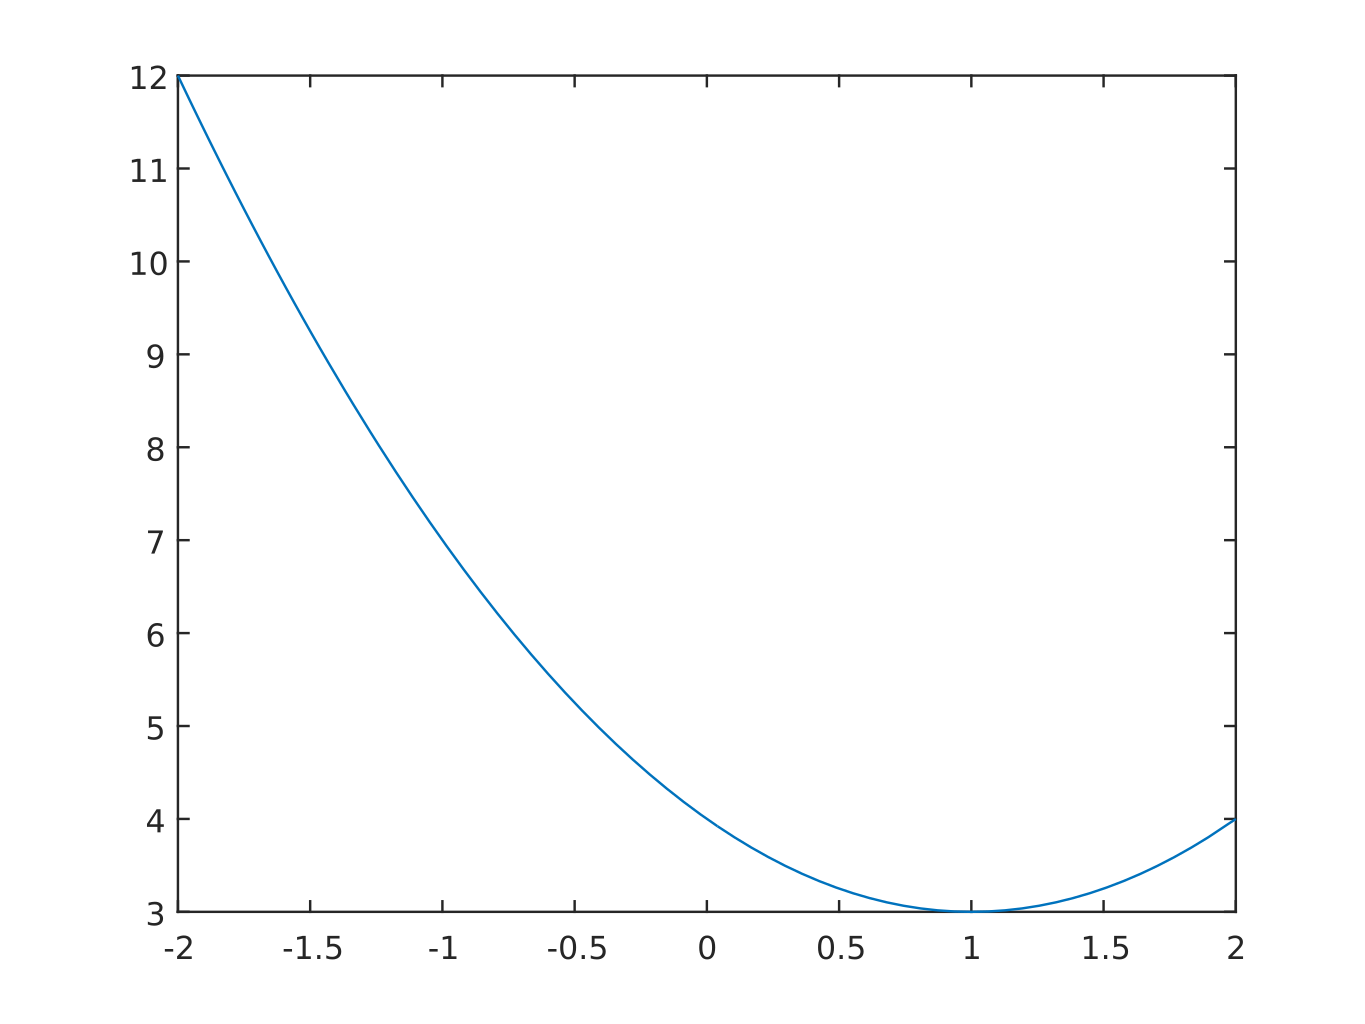
\includegraphics[width=0.8\columnwidth]{parabola.png}
                \caption{Parabola}
            \end{figure}\noindent

        \subsection{Podpunkt f}
\begin{lstlisting}
Imie = {'Rafał' 'Monika', 'Paweł', 'Elżbieta', 'Mirek'}
Matematyka = [36, 83, 2, 5, 17]';       
Fizyka = [65, 74, 65, 46, 55]';
Chemia = [30, 75, 19, 69, 19]';

T = table(Matematyka, Fizyka, Chemia,'RowNames',Imie)

writetable(T, 'moje.csv')

%                Matematyka    Fizyka    Chemia
%                __________    ______    ______
%
%    Rafał       36            65        30    
%    Monika      83            74        75    
%    Paweł        2            65        19    
%    Elżbieta     5            46        69    
%    Mirek       17            55        19    
\end{lstlisting}
\end{document}
